
\documentclass[xcolor={table,dvipsnames}]{beamer}

\usetheme{Warsaw}

\usepackage[utf8]{inputenc}
\usepackage[frenchb]{babel}
\usepackage[T1]{fontenc}
\usepackage{amsmath}
\usepackage{hyperref}


\usepackage{graphicx}

\usepackage{tikz}
\usetikzlibrary{arrows}

\pdfcompresslevel0

\newcommand{\camljava}{{\tt{camljava}}}

\usepackage{listings}
\usepackage{color}
\definecolor{darkgray}{rgb}{.5,.2,.2}

\usepackage[table]{xcolor}

\lstdefinelanguage{idlgrammar}{
  morekeywords={package,abstract,extends,class,implements,static,final,<ini>,interface,callback,array,[,],{,},
    name ,void,boolean,byte,char,short,int,long,float,double,string},
  alsoletter=[]{},
}
\lstnewenvironment{idlEx}
                  {\lstset{
                      language=idlgrammar,
                      breaklines=true,
                      showstringspaces=false,
                      commentstyle=\color{red},
                      stringstyle=\color{darkgray},
                      identifierstyle=\ttfamily\textit,
                      keywordstyle=\color{blue},
                      basicstyle=\tiny,
                      escapeinside={/*}{*/},
                      frame=single,
                      %xleftmargin=0.08\textwidth
                    }
                  }
                  {}

\lstnewenvironment{OCamlEx}
                  {\lstset{
                      language=[Objective]Caml,
                      breaklines=true,
                      showstringspaces=false,
                      commentstyle=\color{red},
                      stringstyle=\color{darkgray},
                      identifierstyle=\ttfamily,
                      keywordstyle=\color{blue},
                      basicstyle=\tiny,
                      escapeinside={/*}{*/},
                      frame=single,
                      %xleftmargin=0.08\textwidth
                    }
                  }
                  {}

\lstnewenvironment{javaEx}
                  {\lstset{
                      language=Java,             
                      breaklines=true,
                      showstringspaces=false,
                      commentstyle=\color{red},
                      stringstyle=\color{darkgray},
                      identifierstyle=\ttfamily\textit,
                      keywordstyle=\color{purple},
                      basicstyle=\tiny,
                      escapeinside={/*}{*/},
                      frame=double,
                      %xleftmargin=0.08\textwidth
                    }
                  }
                  {}


\addtobeamertemplate{footline}{\hfill\insertframenumber/\inserttotalframenumber

\hspace{10em}\\}

\usepackage{listings}

\title{Interopérabilité entre OCaml et Java }
\author{Béatrice Carré}
\date{\today}

% slides number
\defbeamertemplate*{footline}{shadow theme}
{%
  \leavevmode%
  \hbox{
    \begin{beamercolorbox}[wd=.5\paperwidth,ht=2.5ex,dp=1.125ex,leftskip=.3cm plus1fil,rightskip=.3cm]{author in head/foot}%
    \usebeamerfont{author in head/foot}\insertframenumber\,/\,\inserttotalframenumber\hfill\insertshortauthor
  \end{beamercolorbox}%
  \begin{beamercolorbox}[wd=.5\paperwidth,ht=2.5ex,dp=1.125ex,leftskip=.3cm,rightskip=.3cm plus1fil]{}%
    \usebeamerfont{title in head/foot}\insertshorttitle%
  \end{beamercolorbox}}%
  \vskip0pt%
}

\beamertemplatenavigationsymbolsempty


\begin{document}

\maketitle




\begin{frame}{Objectif}
\begin{definition}
L'\alert{interop\'erabilit\'e entre deux langages} est la 
capacité d'un programme écrit dans un certain langage d'utiliser un
programme dans un autre langage.
\end{definition}
\begin{itemize}
\item \textbf{Intérêt} :

Tirer parti des spécificités de chaque langage.

\item\textbf{Interopérabilité efficace} :

 Accès simple à l'autre langage (ici, manipuler un objet Java comme un
 objet OCaml.

\item \textbf{Projet} : 
  
  Adapter deux travaux déjà développés (\emph{O'Jacaré} et \emph{OCaml-Java}) pour tirer parti des avantages de chacun.

\end{itemize}
\end{frame}



\begin{frame}{Comparaison des deux mondes}
Dans ce projet, l'interopérabilité se fait sur le modèle objet de
chacun :

\bigskip
\begin{tabular}{|l|c|c|c|c|}
  \hline \rowcolor[gray]{0.9}
  \emph{caractéristiques} & \emph{Java} & \emph{OCaml} \\
  \hline
  accès champs & selon la visibilité & via appels de méthode\\\hline
  var./méth. statiques & \checkmark & fonct./décl. globales\\\hline
  typage dynamique & \checkmark &  $\times$  \\\hline
  surcharge & \checkmark & $\times$ \\\hline
  héritage multiple & pour les interfaces & \checkmark\\
  \hline
\end{tabular}

\bigskip

\begin{definition}
Une \alert{interface} définit la frontière de communication entre deux
entités.
\end{definition}
Pour l'interopérabilité, il est nécessaire de définir une interface qui adapte les deux modèles.
\end{frame}



\begin{frame}{O'Jacaré : schéma global }

\begin{definition}
Un \alert{IDL} (Langage de Définition d'Interface) définit une interface entre les deux langages, qui va permettre de les faire communiquer.
\end{definition}

O'Jacaré génère les classes encapsulantes à partir d'un IDL dans lequel sont décrites les classes qu'on veut manipuler.
\medskip
\begin{figure}[h]
  \centering
  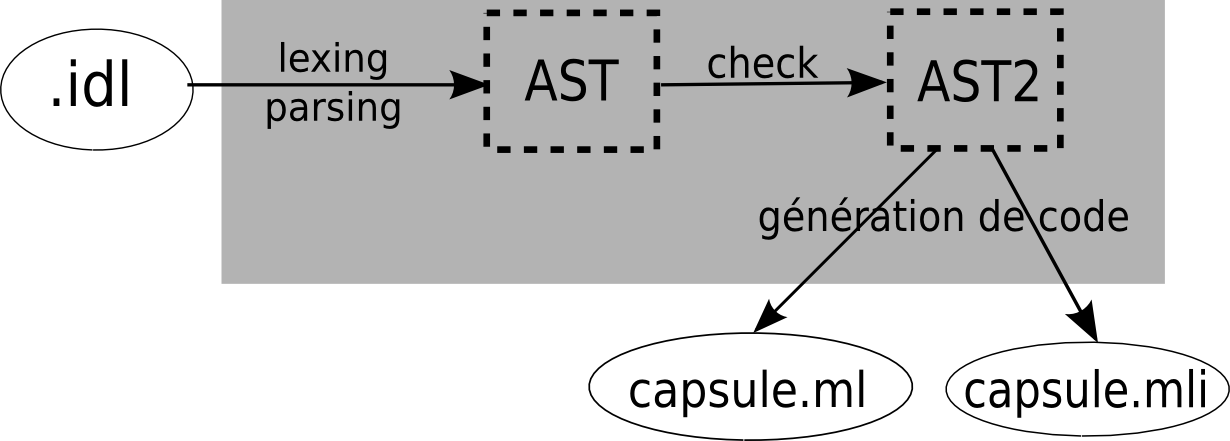
\includegraphics[scale=0.9]{schemaOjacare.png}
\end{figure}

\end{frame}


\begin{frame}{O'Jacaré : schéma global (2) }
  \begin{definition}
    La \alert{classe encapsulante} générée à partir de l'IDL contient une référence sur un objet Java et permet à l'utilisateur de faire les appels sur celui-ci.
  \end{definition}
La bibliothèque \camljava \ gère la communication OCaml-Java :
\begin{itemize}
\item Recherche des classes par nom et des méthodes par signature
\item Conversion des types de base
\end{itemize}
\begin{figure}[h!]
  \centering
  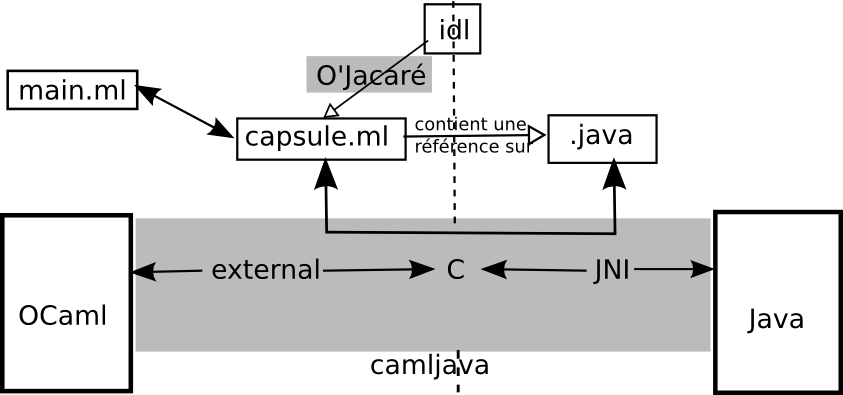
\includegraphics[scale=0.8]{schemaCamljava2.png}
\end{figure}

\end{frame}





\begin{frame}[fragile]{O'Jacaré exemple : La classe Point (Java)}
%mise en page TODO

\bigskip

\begin{javaEx} 
  package mypack;
  public class Point {
    int x;
    int y;
    public Point() { 
      this.x = 0;
      this.y = 0;
    }
    public Point(int x,int y) {
      this.x = x;
      this.y = y;
    }
    public void moveto(int x,int y){
      this.x = x;
      this.y = y;
    }
    public String toString() {
      return "("+x+","+y+")";
    }
    public double distance() {
      return Math.sqrt (this.x*this.x+this.y*this.y);
    }
    public boolean eq(Point p) {
      return this.x == p.x  && this.y == p.y;
    }
  }
\end{javaEx}

\end{frame}





\begin{frame}[fragile]{O'Jacaré exemple : IDL et utilisation}
  IDL : point.idl
\begin{idlEx} 
package mypack;

class Point {
  int x;
  int y; 
  [name default_point] <init> ();
  [name point] <init> (int,int);
  void moveto(int,int);
  string toString();
  boolean eq(Point);
}
\end{idlEx}

Utilisation : main.ml
\begin{OCamlEx}
  open Point

  let p = new default_point () in
  let p2 = new point 1 1 in
  p#moveto 4 3;
  p#tostring ();
  print_string (if (p#eq p2) then "true" else "false")
\end{OCamlEx}
\end{frame}




\begin{frame}{OCaml-Java : schéma global}
\begin{figure}[h!]
  \centering
  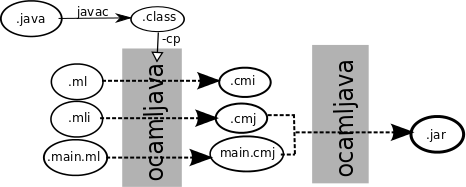
\includegraphics[scale=0.8]{schemaOCamlJava.png}
\end{figure}
Compilation vers du bytecode Java

$\Rightarrow$ un seul runtime
\begin{itemize}
\item Pas de problème de gestion mémoire
\item Typage statique
\end{itemize}
\end{frame}





\begin{frame}[fragile]{OCaml-Java : l'accès au monde Java}

  Accès à du code Java grâce à des méthodes définies dans le
  \textbf{module Java} OCaml pour OCaml-Java.

\bigskip

Exemple d'utilisation :

\begin{OCamlEx}
and x = Int32.of_int 1
and y = Int32.of_int 2 in
let (p : mypack'Point java_instance) = 
   Java.make "mypack.Point()" ()
let (p2 : mypack'Point java_instance) = 
   Java.make "mypack.Point(int,int)" x y 
in
   Java.call "mypack.Point.eq(mypack.Point):boolean" p p2
\end{OCamlEx}

\end{frame}


\begin{frame}{Fusion des deux approches}

\begin{tabular}{|c|c@{\,\vrule width 6pt\,}c|}
  \hline
   \cellcolor[gray]{0.6}\emph{O'Jacaré+}\camljava & \cellcolor[gray]{0.6}\emph{OCaml-Java}& \cellcolor[gray]{0.6} \emph{O'Jacaré+OCaml-Java}\\
  \hline\hline
 \cellcolor[gray]{0.8} appels transparents & via module Java & \cellcolor[gray]{0.8}appels transparents\\
\hline
  2 runtimes &\cellcolor[gray]{0.8} 1 runtime&\cellcolor[gray]{0.8} 1 runtime \\
\hline
\end{tabular}

\bigskip 

\begin{figure}[h]
  \centering
  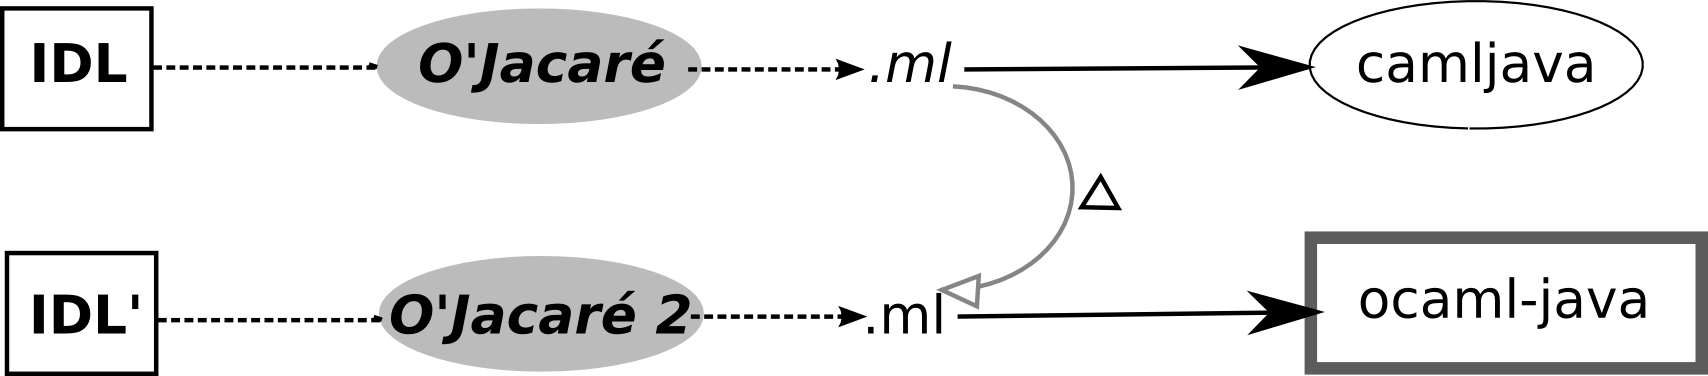
\includegraphics[scale=1]{schema1.png}
\end{figure}

\end{frame}



\begin{frame}{Adaptation d'Ojacaré : O'Jacaré 2}

\begin{enumerate}
\item Garder la même structure de capsule sauf l'introspection des
  types dynamiques, qui se fait statiquement par OCaml-Java

\item Adapter au module \emph{Java} de OCaml-Java

\item Redéfinir la conversion des types

\begin{figure}\scalebox{0.8}{
\centering
\begin{tabular}{|c|l|l|l|}
 \hline
 \rowcolor[gray]{0.8}
\emph{TYPE IDL} & \emph{type Java} &\emph{type OCaml manipulés} &
\emph{type OCaml} \\ 
\rowcolor[gray]{0.8}
& (java\_type) & \emph{par OCaml-Java} (oj\_type t) & (ml\_type t)\\
 \hline
\emph{int} & int & int32 & int\\
\emph{long} & long & int64 & int\\
\emph{string} & java.lang.String & java'lang'String java\_instance & string\\
\emph{pack/Obj} & pack.Obj & pack'Obj java\_instance & jObj\\
 \hline
\end{tabular}
}
\end{figure}

\end{enumerate}
\end{frame}





\begin{frame}[fragile]{Comparaison de génération}

La génération du constructeur de Point par 
\begin{itemize}
\item O'Jacaré
\begin{OCamlEx}
let _init_point =
  let clazz = Jni.find_class "mypack/Point" in
  let id =
    try Jni.get_methodID clazz "<init>" "(II)V"
    with | _ ->failwith
          "Unknown constructor from IDL in class \"mypack.Point\" : \"Point(int,int)\"."
  in
    fun (java_obj : _jni_jPoint) _p0 _p1 ->
      let _p1 = _p1 in
      let _p0 = _p0
      in
        Jni.call_nonvirtual_void_method java_obj clazz id
          [| Jni.Camlint _p0; Jni.Camlint _p1 |];;
class point _p0 _p1 =
  let java_obj = _alloc_jPoint ()
  in let _ = _init_point java_obj _p0 _p1
    in object (self) inherit _capsule_jPoint java_obj end;;
\end{OCamlEx}

\item O'Jacaré 2 
\begin{OCamlEx}
class point _p0 _p1 =
  let _p1 = Int32.of_int _p1
  in let _p0 = Int32.of_int _p0
    in let java_obj = Java.make "mypack.Point(int,int)" _p0 _p1
      in object (self) inherit _capsule_jPoint java_obj end;;
\end{OCamlEx}

\end{itemize}
\end{frame}


\begin{frame}{Conclusion}

Travail :
\begin{itemize}
\item S'approprier les outils et lire les articles associés
\item Comprendre le système de types de OCaml-Java
\item Ecrire O'Jacaré 2
\end{itemize}

O'Jacaré 2 :
\begin{itemize}
\item Accès simple à du code Java ou à l'API
\item Accès utilisateur transparent grâce aux classes encapsulantes
\item 1 seul runtime -> gestion mémoire plus sûre
\item Code généré simplifié ($\sim$ 5 fois moins de lignes)
\end{itemize}

Travaux futurs:
\begin{itemize}
\item Conversion des types tableaux
\item Gérer un mécanisme de rappel (la redéfinition d'une méthode Java
  pas une méthode OCaml)
\end{itemize}
\end{frame}





\begin{frame}{Bibliographie}

  \begin{thebibliography}{}
  \bibitem{DAOC} CHAILLOUX E., MANOURY P., PAGANO B., \emph{Développement
    d'applications avec Objective Caml}, O'Reilly
    , 2000

  \bibitem{}  HENRY G., \emph{O’Jacaré} \url{http://www.pps.univ-paris-diderot.fr/~henry/ojacare/}

  \bibitem{}  CLERC X.,\emph{OCaml-Java 2.0} \url{http://ocamljava.x9c.fr/preview/}

  \bibitem{} CHAILLOUX E., HENRY G., \emph{O’Jacaré, une interface objet
    entre Objective Caml et Java}, 2004

  \bibitem{} CLERC X., \emph{OCaml-Java: Typing Java Accesses from OCaml
    Programs}, Trends in Functional Programming, Lecture Notes in
    Computer Science Volume 7829,
    2013

  \bibitem{camljava} Leroy X., \emph{The camljava project},

  \bibitem{module Java} CLERC X.,\emph{OCaml-java : module Java} \href{http://ocamljava.x9c.fr/preview/javalib/index.html}{lien}

  \end{thebibliography}
\end{frame}



\begin{frame}[fragile]{Module Java de OCaml}
\scalebox{0.8}{
\begin{tabular}{|l|l|}
  \hline
  \emph{types OCaml-Java} & \emph{descriptions et exemples} \\\hline
  java\_instance & référence sur une instance Java  \\
  \hline
  java\_constructor & signature d'un constructeur  \\
  &  "java.lang.Object()" \\
  \hline
  java\_method & signature d'une méthode \\
  & "java.lang.String.lastIndexOf(String):int"\\
  \hline
  java\_field\_get & signature d'un attribut\\
  & "mypack.Point.x:int" \\
  \hline
  java\_field\_set & signature d'un attribut\\
  & "mypack.Point.x:int" \\
  \hline
  java\_type & classe, interface ou type Array\\
  & "java.lang.String"\\
  \hline
\end{tabular}
}
\begin{OCamlEx}
/*\textbf{make}*/ : 'a java_constructor -> 'a 
/*\textbf{call}*/ : 'a java_method -> 'a 
/*\textbf{get}*/ : 'a java_field_get -> 'a 
/*\textbf{set}*/ : 'a java_field_set -> 'a 
/*\textbf{is\_null}*/ : 'a java_instance -> bool 
/*\textbf{instanceof}*/ : 'a java_type -> 'b java_instance -> bool
/*\textbf{cast}*/ : 'a java_type -> 'b java_instance -> 'a
\end{OCamlEx}
\end{frame}


\begin{frame}[fragile]{génération O'Jacaré 2 : la classe Point}
\begin{OCamlEx}
type top = java'lang'Object java_instance;;
exception Null_object of string;;
type _jni_jPoint = mypack'Point java_instance;;
class type jPoint =
  object
    method _get_jni_jPoint : _jni_jPoint
    method set_x : int -> unit
    method get_x : unit -> int
    method set_y : int -> unit
    method get_y : unit -> int
    method moveto : int -> int -> unit
    method toString : unit -> string
    method eq : jPoint -> bool
  end;;
class _capsule_jPoint (jni_ref : _jni_jPoint) =
  let _ =
    if Java.is_null jni_ref then raise (Null_object "mypack/Point") else ()
  in
    object (self)
      method eq =
        fun (_p0 : jPoint) ->
          let _p0 = _p0#_get_jni_jPoint
          in Java.call "mypack.Point.eq(mypack.Point):boolean" jni_ref _p0
      method toString =
        fun () ->
          JavaString.to_string
            (Java.call "mypack.Point.toString():java.lang.String"
          jni_ref)
\end{OCamlEx}
\end{frame}

\begin{frame}[fragile]{génération O'Jacaré 2 : la classe Point (2)}
\begin{OCamlEx}
      method moveto =
        fun _p0 _p1 ->
          let _p1 = Int32.of_int _p1 in
          let _p0 = Int32.of_int _p0
          in Java.call "mypack.Point.moveto(int,int):void" jni_ref _p0 _p1
      method set_y =
        fun _p ->
          let _p = Int32.of_int _p
          in Java.set "mypack.Point.y:int" jni_ref _p
      method get_y =
        fun () -> Int32.to_int (Java.get "mypack.Point.y:int" jni_ref)
      method set_x =
        fun _p ->
          let _p = Int32.of_int _p
          in Java.set "mypack.Point.x:int" jni_ref _p
      method get_x =
        fun () -> Int32.to_int (Java.get "mypack.Point.x:int" jni_ref)
      method _get_jni_jPoint = jni_ref
    end;;
let jPoint_of_top (o : top) : jPoint =
  new _capsule_jPoint (Java.cast "mypack.Point" o);;
let _instance_of_jPoint (o : top) = Java.instanceof "mypack.Point" o;;
class point _p0 _p1 =
  let _p1 = Int32.of_int _p1
  in let _p0 = Int32.of_int _p0
    in let java_obj = Java.make "mypack.Point(int,int)" _p0 _p1
      in object (self) inherit _capsule_jPoint java_obj end;;
class default_point () =
  let java_obj = Java.make "mypack.Point()" ()
  in object (self) inherit _capsule_jPoint java_obj end;;
\end{OCamlEx}
\end{frame}
\end{document}

